\section{Performance Evaluation}
\label{sec:evaluation}
In this section, we evaluate the performance of the proposed low-complexity dispatching policy $\tilde{\Policy}$ by numerical simulations.
The experiment setup and performance benchmarks are elaborated in Section \ref{subsec:setup}.
The simulation results are illustrated in Section \ref{subsec:basic}.
The sensitivity study on parameters is also applied to provide some insights on the robustness of the proposed policy in Section \ref{subsec:advance}.

\subsection{Experiment Setup}
\label{subsec:setup}
In the simulation, we assume that there are $K=15$ APs, $M=10$ processing servers and $J=10$ types of jobs in the system.
One broadcast interval is consist of $t_{B}=25$ time slots.
% The time slot duration is $20$ milliseconds and one broadcast interval consists of $t_{B}=25$ time slots.
The network topology among APs is generated according to Barab\'asi-Albert (BA) model \cite{albert1999diameter} and the processing servers are randomly placed collocated with the APs.
Under this network topology setup with degree as $3$, the subset partition algorithm \ref{alg_0} could reduce the update period $N$ from $15$ to $6$ timeslots.
% The BA model is parameterized by $n$ and $m$ and produces a graph with $n$ vertices and $m$ edges such that the degree distribution follows a power-law.
The arrival traces and job processing time for each job type are extracted from Google cluster traces \cite{clusterdata:Reiss2011} and then randomly assigned on APs and edge servers, respectively.
The maximum uploading latency is $\Xi = 3t_B$, and the distribution of $\mathbb{U}_{k,m,j}(\Xi)$ ($\forall k\in\apSet, m\in\esSet_{k}, j\in\jSpace$) is arbitrarily generated within the support $\set{0, 1, \dots, \Xi}$.
The \brlatency~ is with an integer support from $0.7t_B$ to $0.9t_B$ time slots.
Each queue for VMs on edge server is with maximum queue length $L_{max}=50$, i.e., there would be at most $50$ jobs on one edge server.
The discount factor $\gamma$ is $0.95$ and the penalty weight $\beta$ is $120$.

% %-----------------------------------------------------------------------%
% \begin{figure}[ht]                                                      %
%     \centering                                                          %
%     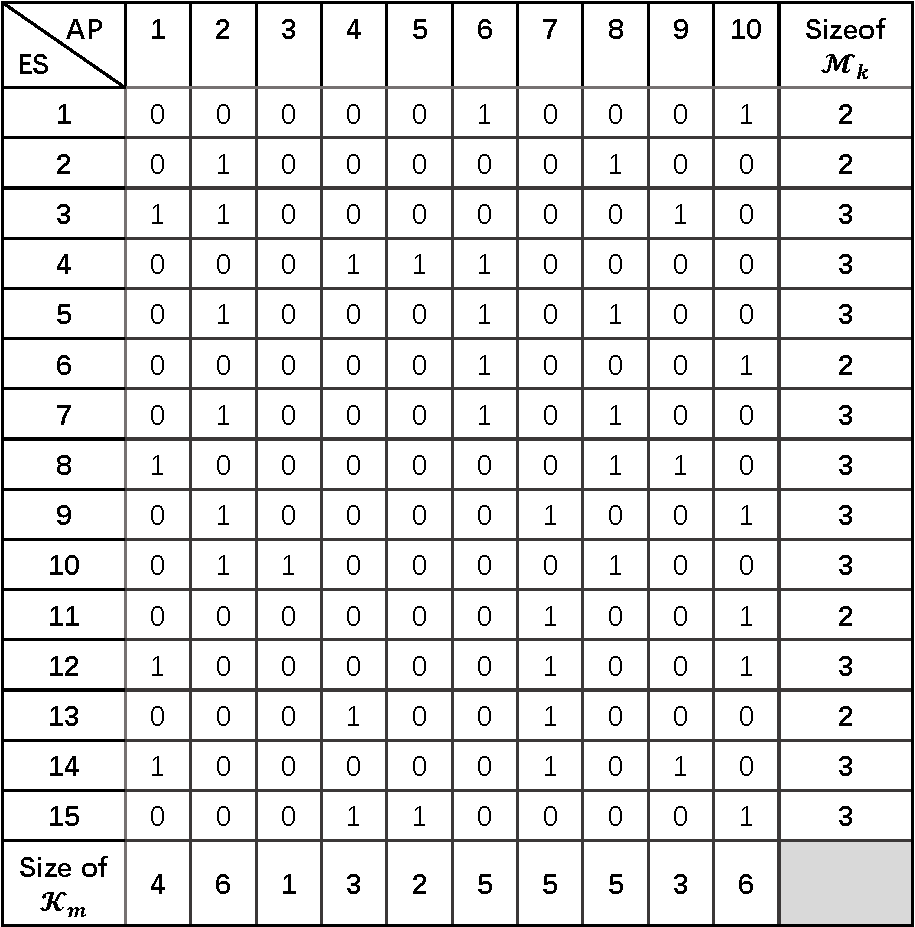
\includegraphics[width=0.45\textwidth]{sim-bipartite.pdf}           %
%     \caption{The illustration of adjacency matrix between APs and edge servers in the simulation.}
%     \label{fig:bipartite}                                               %
% \end{figure}                                                            %
% %-----------------------------------------------------------------------%

%-----------------------------------------------------------------------%
\begin{figure}[ht]                                                      %
    \centering                                                          %
    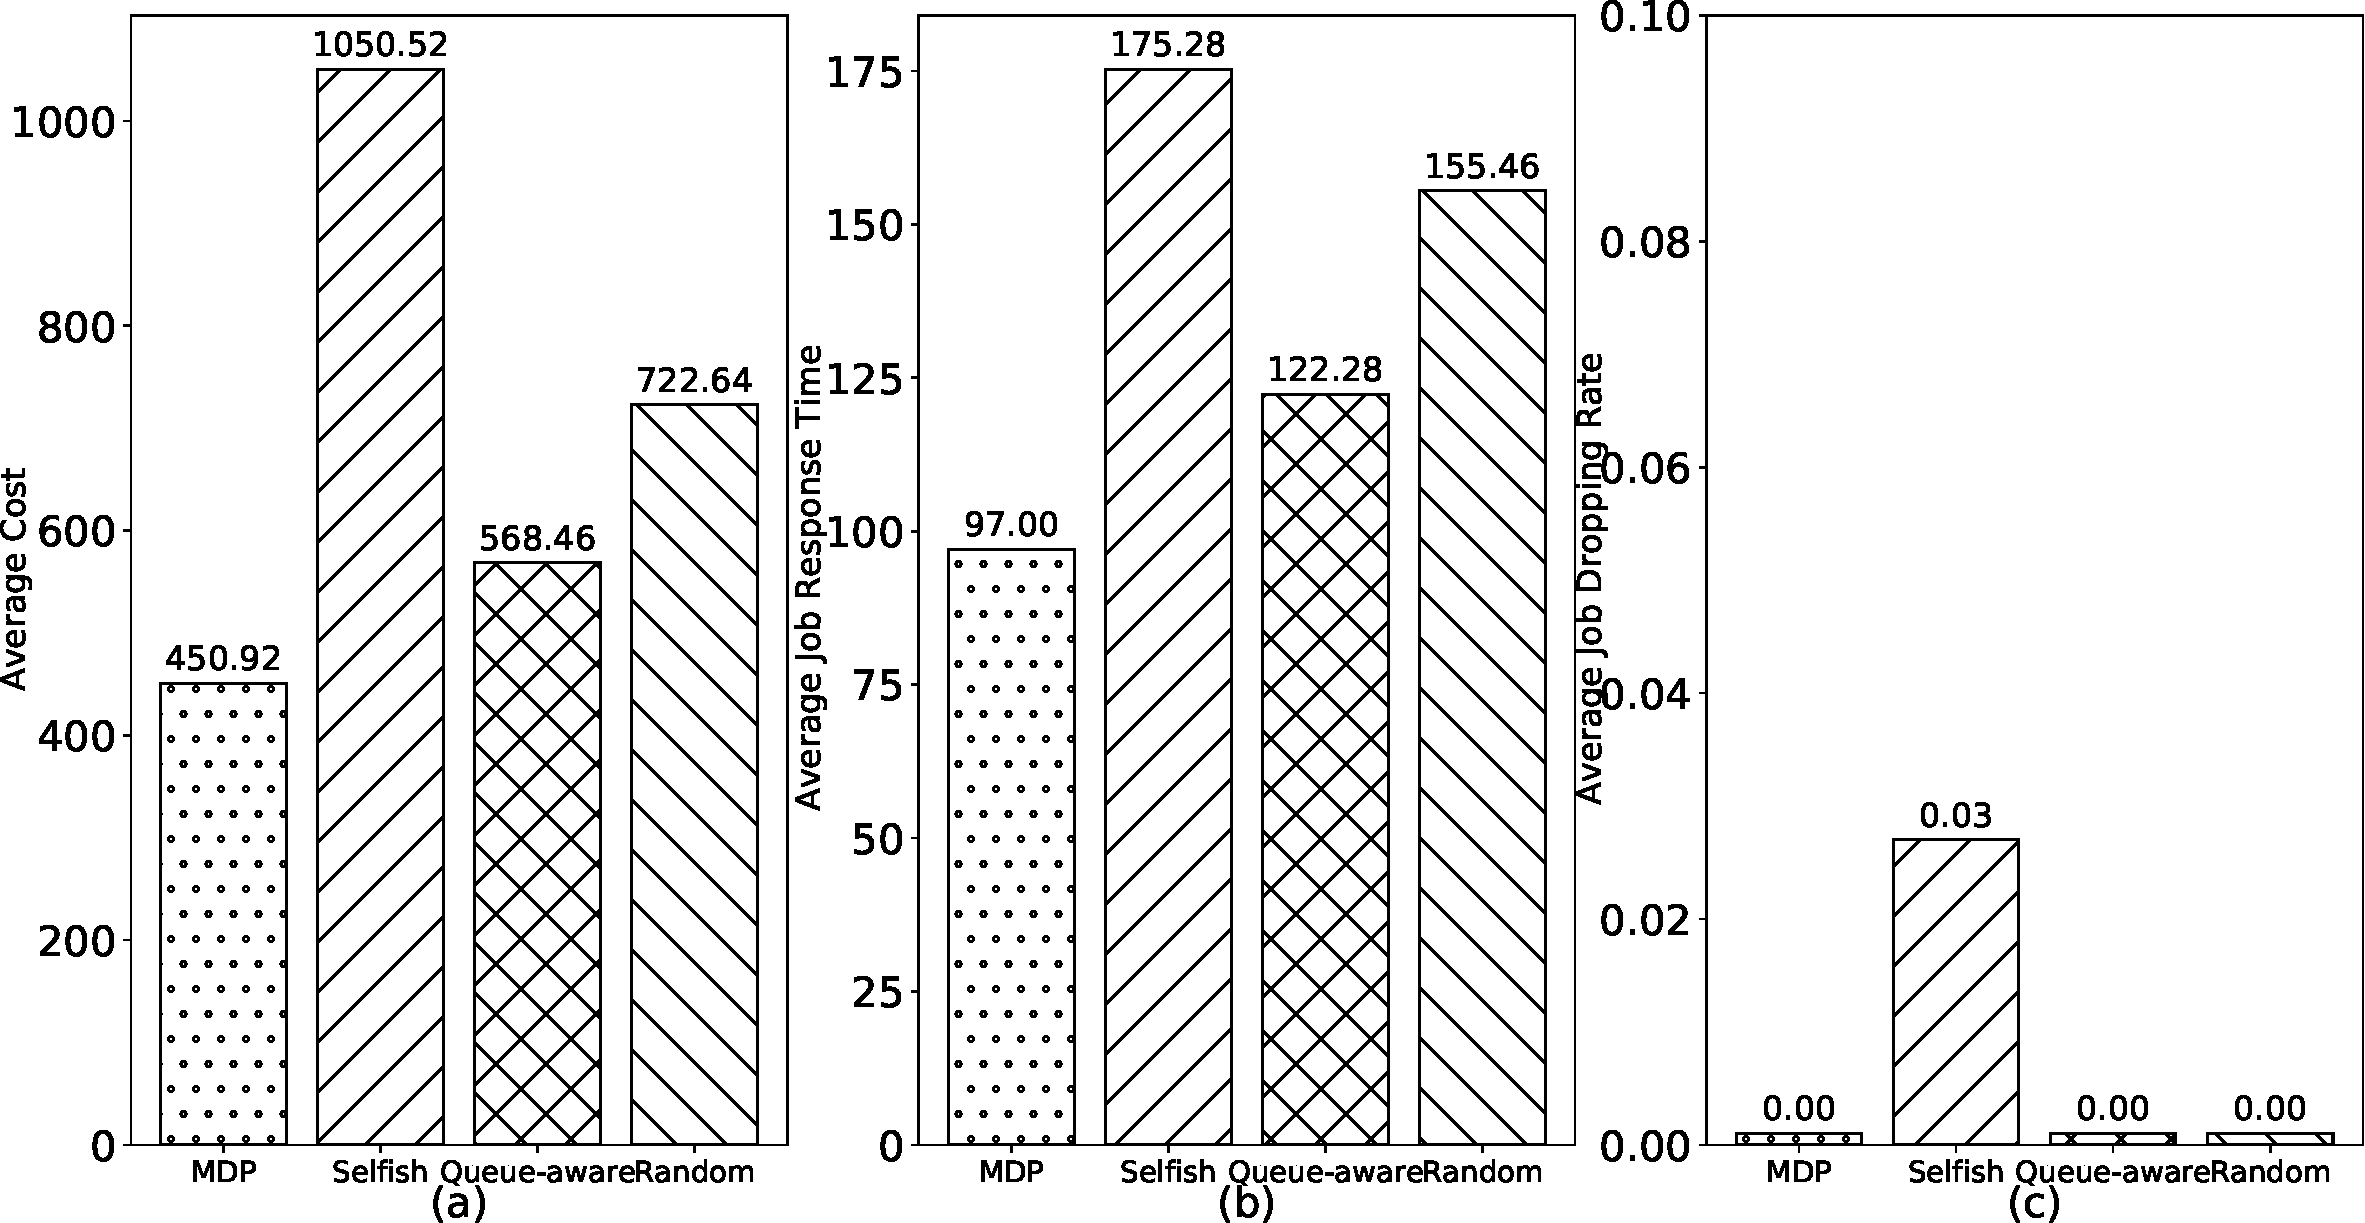
\includegraphics[width=0.45\textwidth]{the-bar-graph-alt.pdf}               %
    \caption{Illustration of performance metrics comparison with benchmarks.}
    \label{fig:bar_plot}                                                %
\end{figure}                                                            %
%-----------------------------------------------------------------------%

%NOTE: Benchmark Elaboration
We also propose {three heuristic benchmarks to profile the performance of the proposed MDP policy}, which are listed as follows.
\begin{itemize}
    \item \textbf{Random Dispatching Policy}:
            Randomly choose a dispatching edge server in each time slot; 
    \item \textbf{Selfish Policy}:
            Always choose the edge server with the minimum sum of the expected uploading time and processing time;
    \item \textbf{Queue-aware Policy}:
            Always choose the edge server with the minimum sum of expected uploading time, processing time and queueing time based on the observation of outdated queue states.
\end{itemize}
Moreover, we choose the Selfish Policy as the initial dispatching actions for our proposed algorithm (Algorithm \ref{alg_1}).

%NOTE: Basic Performance
\subsection{Performance Analysis}
\label{subsec:basic}
As illustrated in Fig.\ref{fig:bar_plot}(a), the proposed algorithm (MDP Policy) outperforms all the benchmarks in the average system cost.
Moreover, the Queue-aware Policy has better performance than the other benchmarks due to its capability of adapting dispatching action according to the outdated observation of queueing state.
More insights on the performance comparison are provided in Fig.\ref{fig:bar_plot}(b) and (c).
In the former figure, the average job response times, measuring the average number of broadcast intervals from job's arrival at one AP to the completeness of computation at one edge server, are compared.
It can be observed that the proposed policy still outperforms all the benchmarks.
In Fig.\ref{fig:bar_plot}(c), the job dropping rates, measuring the ratio of jobs dropped by edge servers due to queue overflow, are also compared.
It is shown that the proposed policy outperforms other three benchmarks with the minimum average cost and job response time.
And there is no dropping jobs incurred compared with the Selfish policy, which is the initial baseline policy for our proposed algorithm.
Finally, an realization of job dispatching is illustrated in Fig.\ref{fig:general_timeline}, where the number of jobs in the system is plot versus the index of broadcast interval.
It can be observed that the proposed policy manage to keep the number of jobs in lower level, compared with the other benchmarks.
This demonstrates its high dispatching efficiency.

%-----------------------------------------------------------------------------------------------%
\begin{figure}[ht!]                                                                             %
    \centering                                                                                  %
    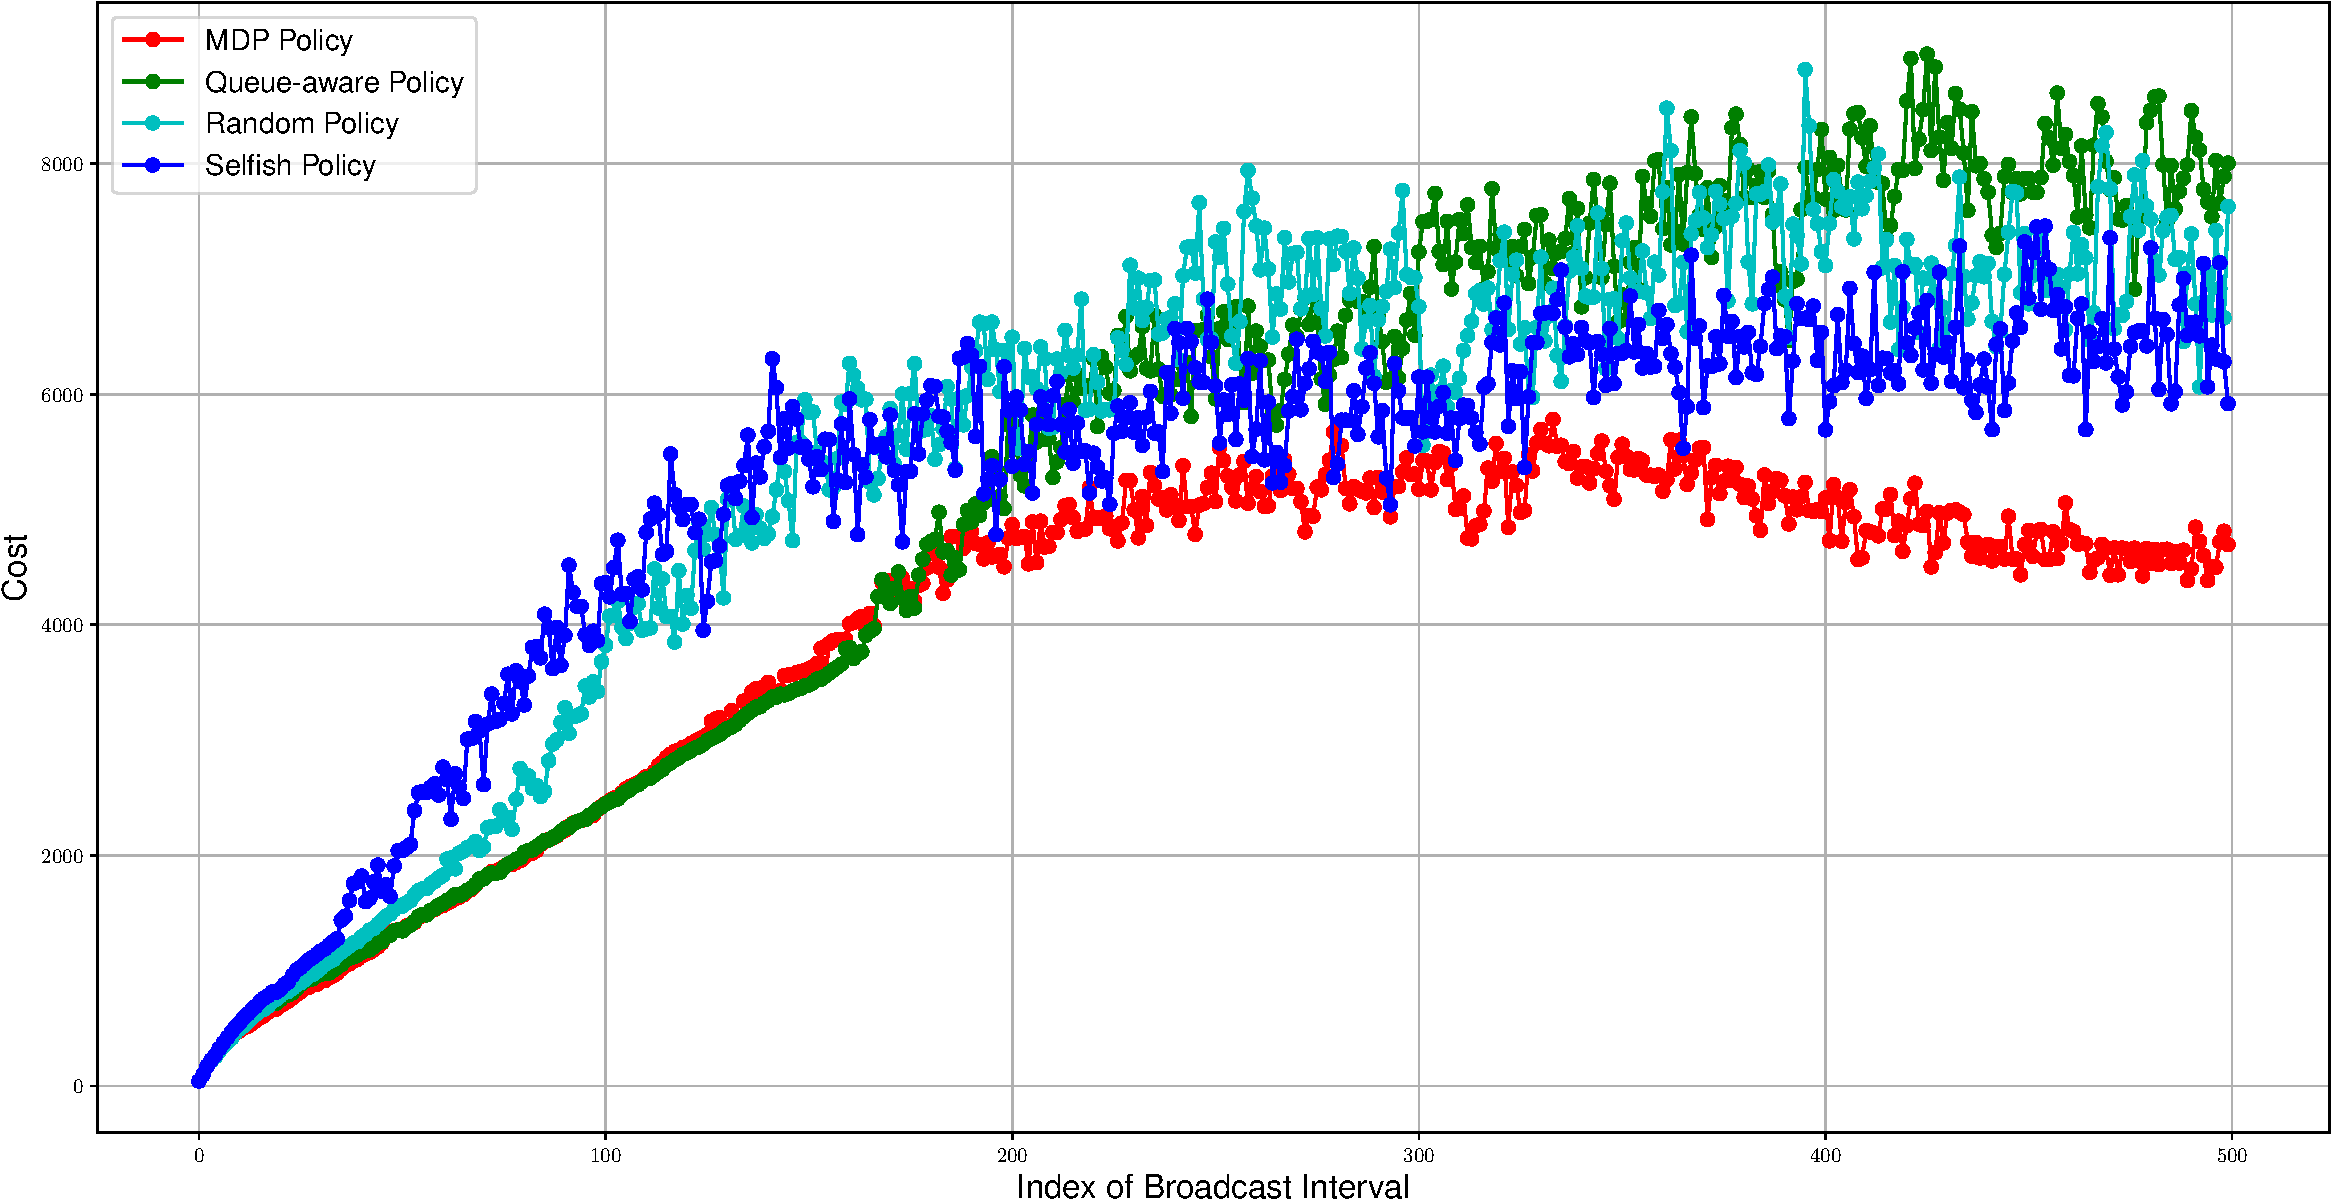
\includegraphics[width=0.45\textwidth]{the-cost-timeline.pdf}                     %
    \caption{Illustration of number of jobs on all the APs and edge servers versus index of broadcast interval.}
    \label{fig:general_timeline}                                                                %
\end{figure}                                                                                    %
%-----------------------------------------------------------------------------------------------%

\subsection{Sensitivity Study}
\label{subsec:advance}
%-----------------------------------------------------------------------------------%
\begin{figure*}[ht!]                                                                %
    \centering                                                                      %
    \begin{minipage}[b]{0.30\textwidth}                                             %
        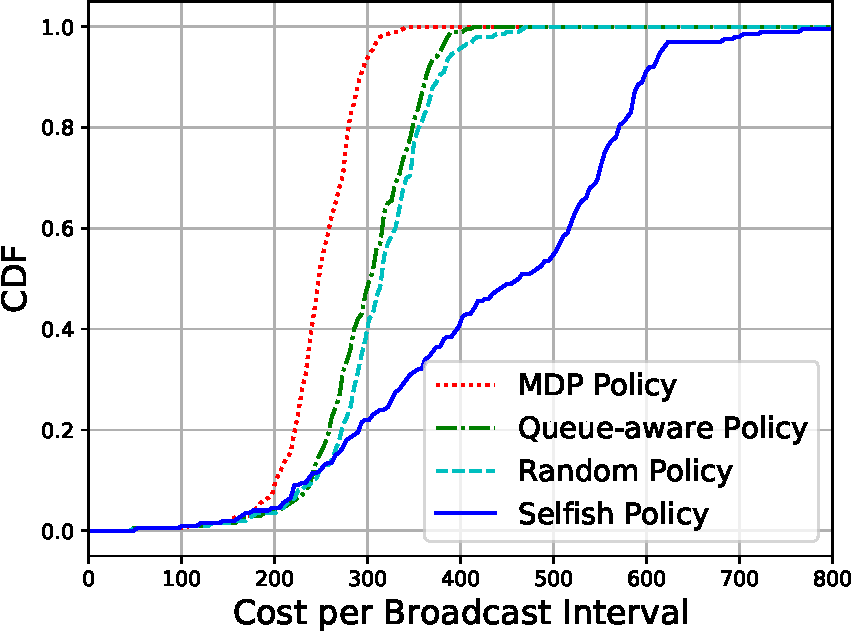
\includegraphics[width=\textwidth]{the-delay-small.pdf} \\                  %
        {(a) \brlatency~as $5$ timeslots.}                                               %
    \end{minipage}                                                                  %
    \begin{minipage}[b]{0.30\textwidth}                                             %
        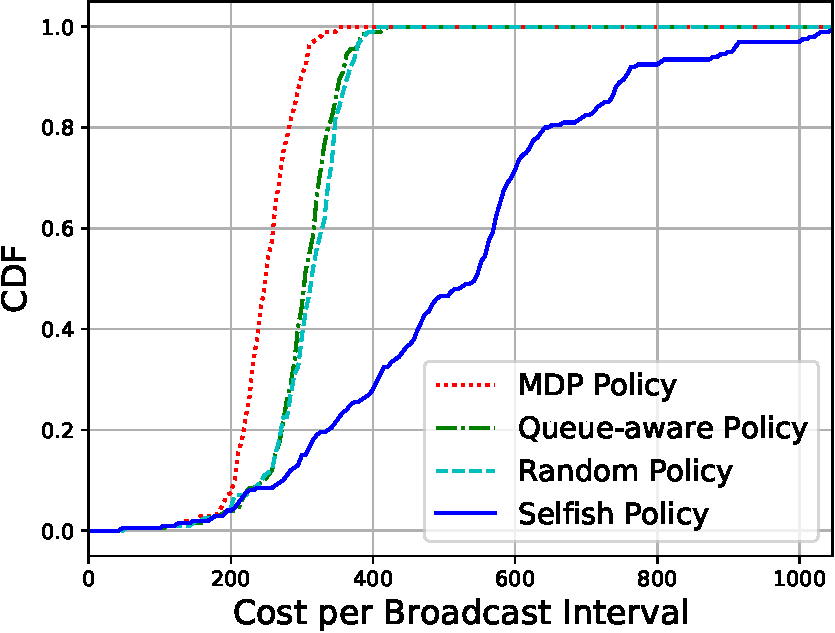
\includegraphics[width=\textwidth]{the-delay-medium.pdf} \\                 %
        {(b) \brlatency~as $12$ timeslots.}           %
    \end{minipage}                                                                  %
    \begin{minipage}[b]{0.30\textwidth}                                             %
        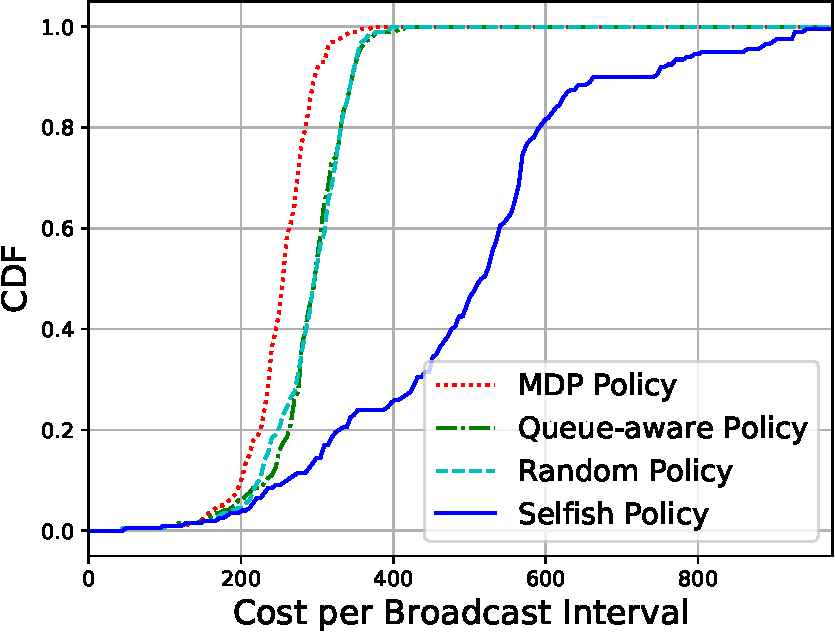
\includegraphics[width=\textwidth]{the-delay-large.pdf} \\                  %
        {(c) \brlatency~as $25$ timeslots.}             %
    \end{minipage}                                                                  %
    \caption{Algorithm Robustness versus Signaling Latency.}                        %
    \label{fig:ss_signal}                                                           %
\end{figure*}                                                                       %
%-----------------------------------------------------------------------------------%

% \begin{figure}[ht!]
%     \centering
%     \begin{minipage}[b]{0.23\textwidth}
%         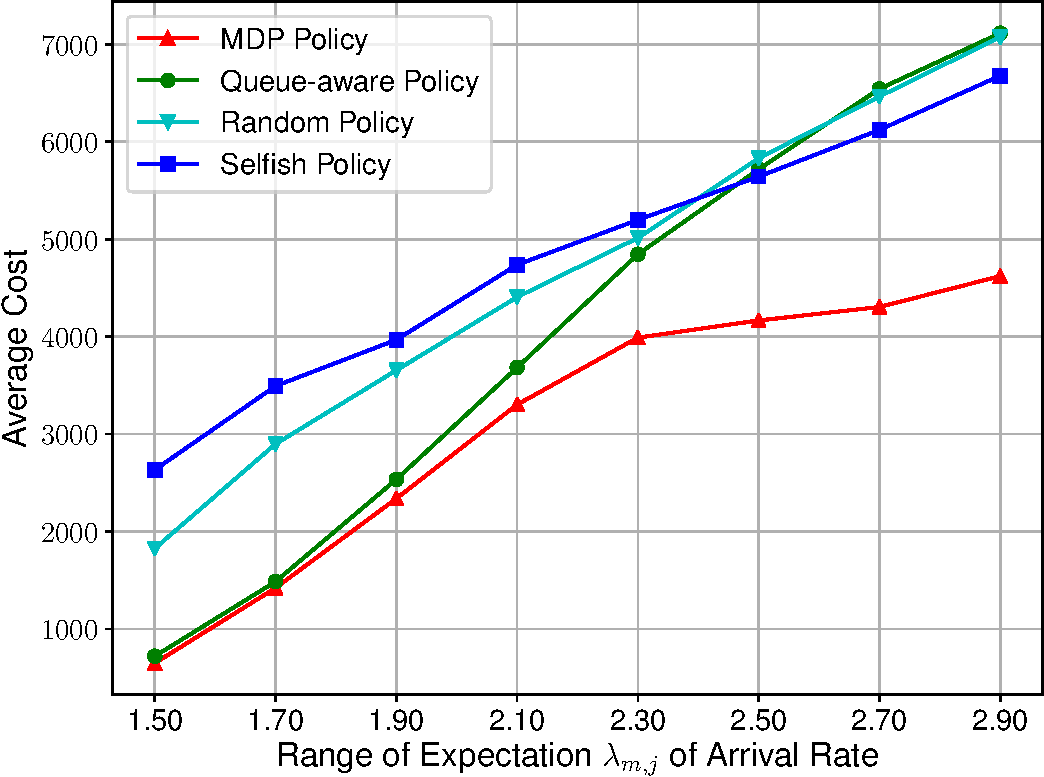
\includegraphics[width=\textwidth]{the-arrival-study.pdf}
%         \caption{Illustration of average system cost versus the number of APs.}
%         \label{fig:ss_scale}
%     \end{minipage}
%     \begin{minipage}[b]{0.23\textwidth}
%         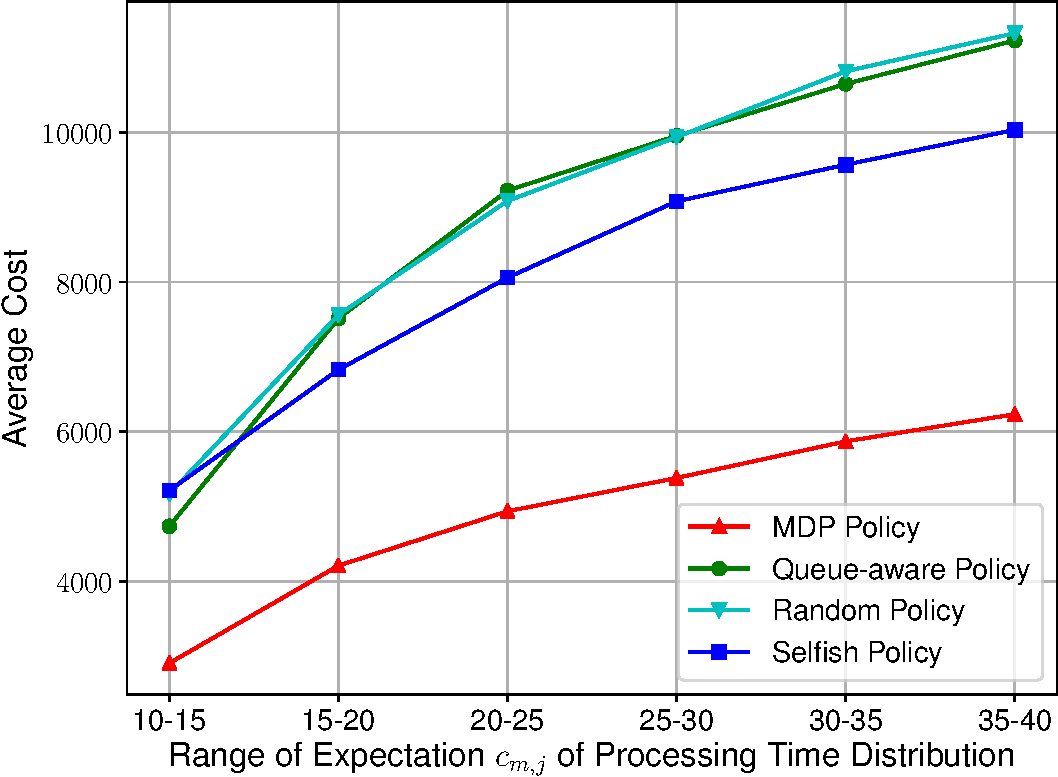
\includegraphics[width=\textwidth]{the-proc-study.pdf}
%         \caption{Illustration of average system cost versus the processing time distributions.}
%         \label{fig:ss_dist}
%     \end{minipage}
% \end{figure}

%-------------------------------------------------------------------%
\begin{figure}[hbt]                                                 %
    \centering                                                      %
    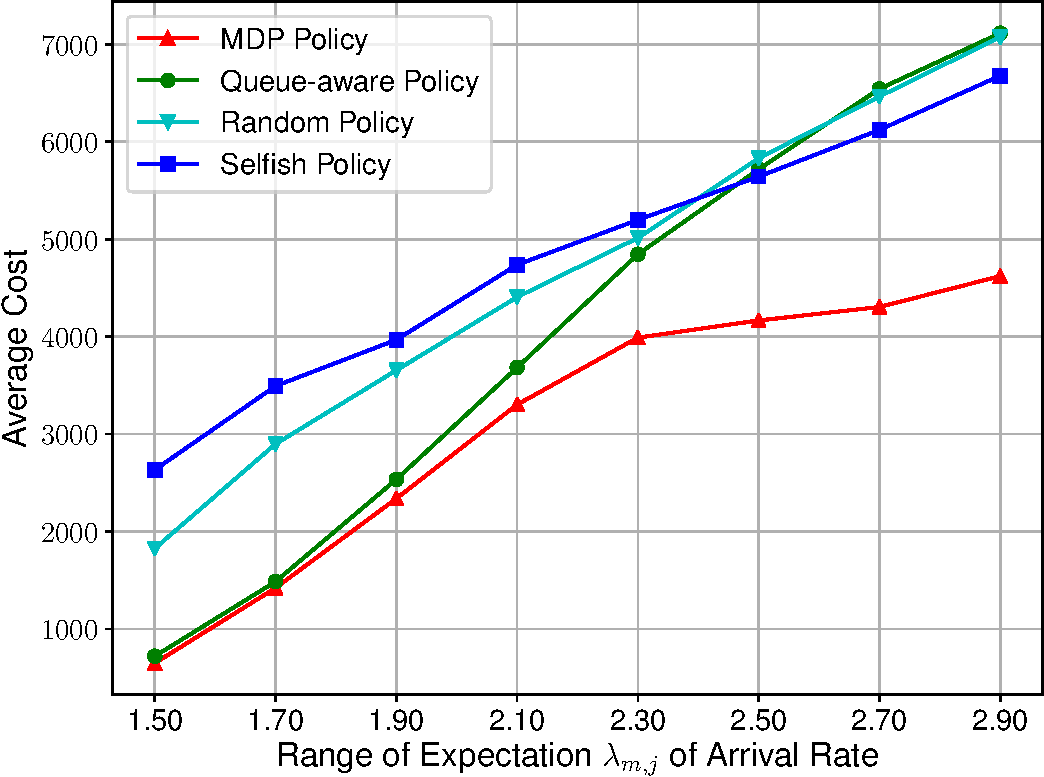
\includegraphics[width=0.45\textwidth]{the-arrival-study.pdf}   %
    \caption{Illustration of average system cost versus the number of APs.}
    \label{fig:ss_scale}                                            %
\end{figure}                                                        %
%-------------------------------------------------------------------%

%-------------------------------------------------------------------%
\begin{figure}[hbt]                                                 %
    \centering                                                      %
    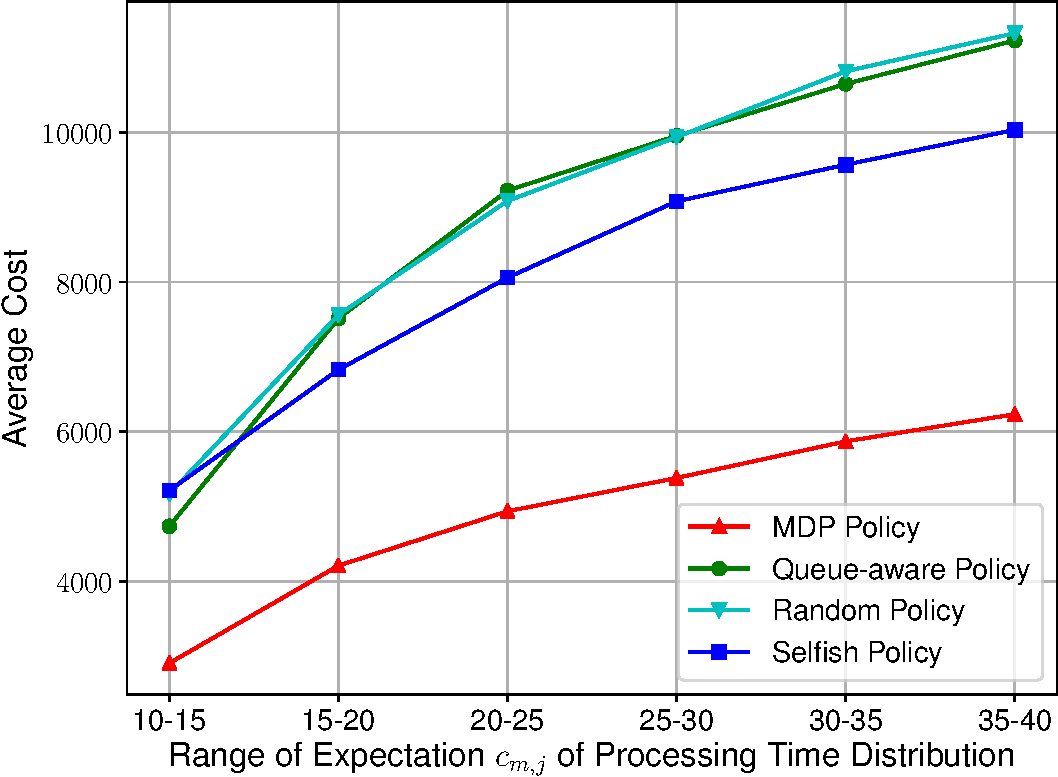
\includegraphics[width=0.45\textwidth]{the-proc-study.pdf}      %
    \caption{Illustration of average system cost versus the mean processing time.}
    \label{fig:ss_dist}                                             %
\end{figure}                                                        %
%-------------------------------------------------------------------%

% %-------------------------------------------------------------------%
% \begin{figure}[hbt]                                                 %
%     \centering                                                      %
%     \includegraphics[width=0.45\textwidth]{bar_graph.pdf}           %
%     \caption{Illustration of impact of penalty factors on algorithms.}
%     \label{fig:ss_penalty}                                          %
% \end{figure}                                                        %
% %-------------------------------------------------------------------%

%NOTE: sensitivity study
\textbf{Signaling Latency.}
The simulation results with different distributions of \brlatency~$\mathcal{D}_{k}$ ($\forall k\in\apSet$) are illustrated in Fig.\ref{fig:ss_signal}, where the cumulative distribution function (CDF) of the job number in the system is plotted.
Specifically, the \brlatency~of all the APs is set to $5, 12, 25$ in Fig.\ref{fig:ss_signal}(a), Fig.\ref{fig:ss_signal}(b) and Fig.\ref{fig:ss_signal}(c), respectively.
It can be observed from Fig.\ref{fig:ss_signal}(a) and Fig.\ref{fig:ss_signal}(c) that, with the increasing \brlatency, the performance of Queue-aware Policy becomes worse.
The Queue-aware policy slightly outperforms the Random Policy in Fig.5(a) with small \brlatency~(achieving a smaller number of jobs in the system), and becomes worse in Fig.5(c) with large \brlatency.
This demonstrates that the Queue-aware Policy is sensitive to the \brlatency.
In all the figures, the proposed policy performs better than the benchmarks, which demonstrates the robustness of its performance versus signaling latency.

\textbf{Job Arrival Intensity.}
We carry out the sensitivity study of arrival intensity by integer scaling the interval of jobs arriving in Google cluster traces.
The average system cost versus the number of APs is illustrated in Fig.\ref{fig:ss_scale}.
With the increasing of job arrival intensity, the average system cost increases in all the benchmarks and our proposed policy.
It can be observed that the proposed policy has better performance than the benchmarks.
Moreover, the performance gain becomes significant when the computation load is heavy.
% This demonstrates the dispatching efficiency of the proposed policy with heavy load.
% The gain is negligible for light load, where the computation capability is sufficient and dispatcher optimization may not be necessary.

\textbf{Mean Processing Time.}
\comments{
The simulation results of various mean processing time are illustrated in Fig.\ref{fig:ss_dist}, where the mean processing time is taken as $c_{m,j}$ of the processing time distribution $\mathbb{G}(1/c_{m,j})$ ($\forall m\in\esSet,j\in\jSpace$) in our computation model assumption.
Generally speaking, with the increasing average processing time, the average system cost increases in all the benchmarks and our proposed policy.
The simulation results are consistent with that in Fig.\ref{fig:ss_scale}.
It can be observed that the proposed policy has better performance than the benchmarks.
Moreover, the performance gain becomes significant when the computation time is long (the computation load is heavy).
% On the other hand, the gain is negligible for short computation time (the computation load is light).
}%

%----------------------------------------------------------------------------------------%

%----------------------------------------------------------------------------------------%